\documentclass[12pt]{article}
{\usepackage{amsmath,amssymb,amsthm,enumerate,dsfont,bm}
\usepackage{pdfpages}
\usepackage[a4paper,bindingoffset=0.2in,%
left=0.8in,right=0.8in,top=1in,bottom=1in,%
footskip=.25in]{geometry}

\newcommand{\prob}[1]{\textbf{P}(#1)}
\newcommand{\ep}[1]{\mathbb{E}\left[ #1 \right]}
\newcommand{\var}[1]{var \left( #1 \right)}
\newcommand{\cp}{\overset{p}{\to}}
\newcommand{\cas}{\overset{a.s.}{\to}}
\newcommand{\cd}{\overset{D}{\to}}
\newcommand{\pard}[1]{\frac{\partial}{\partial #1}}

\title{Statistical Theory Final Solution}
\date{\today}
\author{Bohao Tang}

\begin{document}
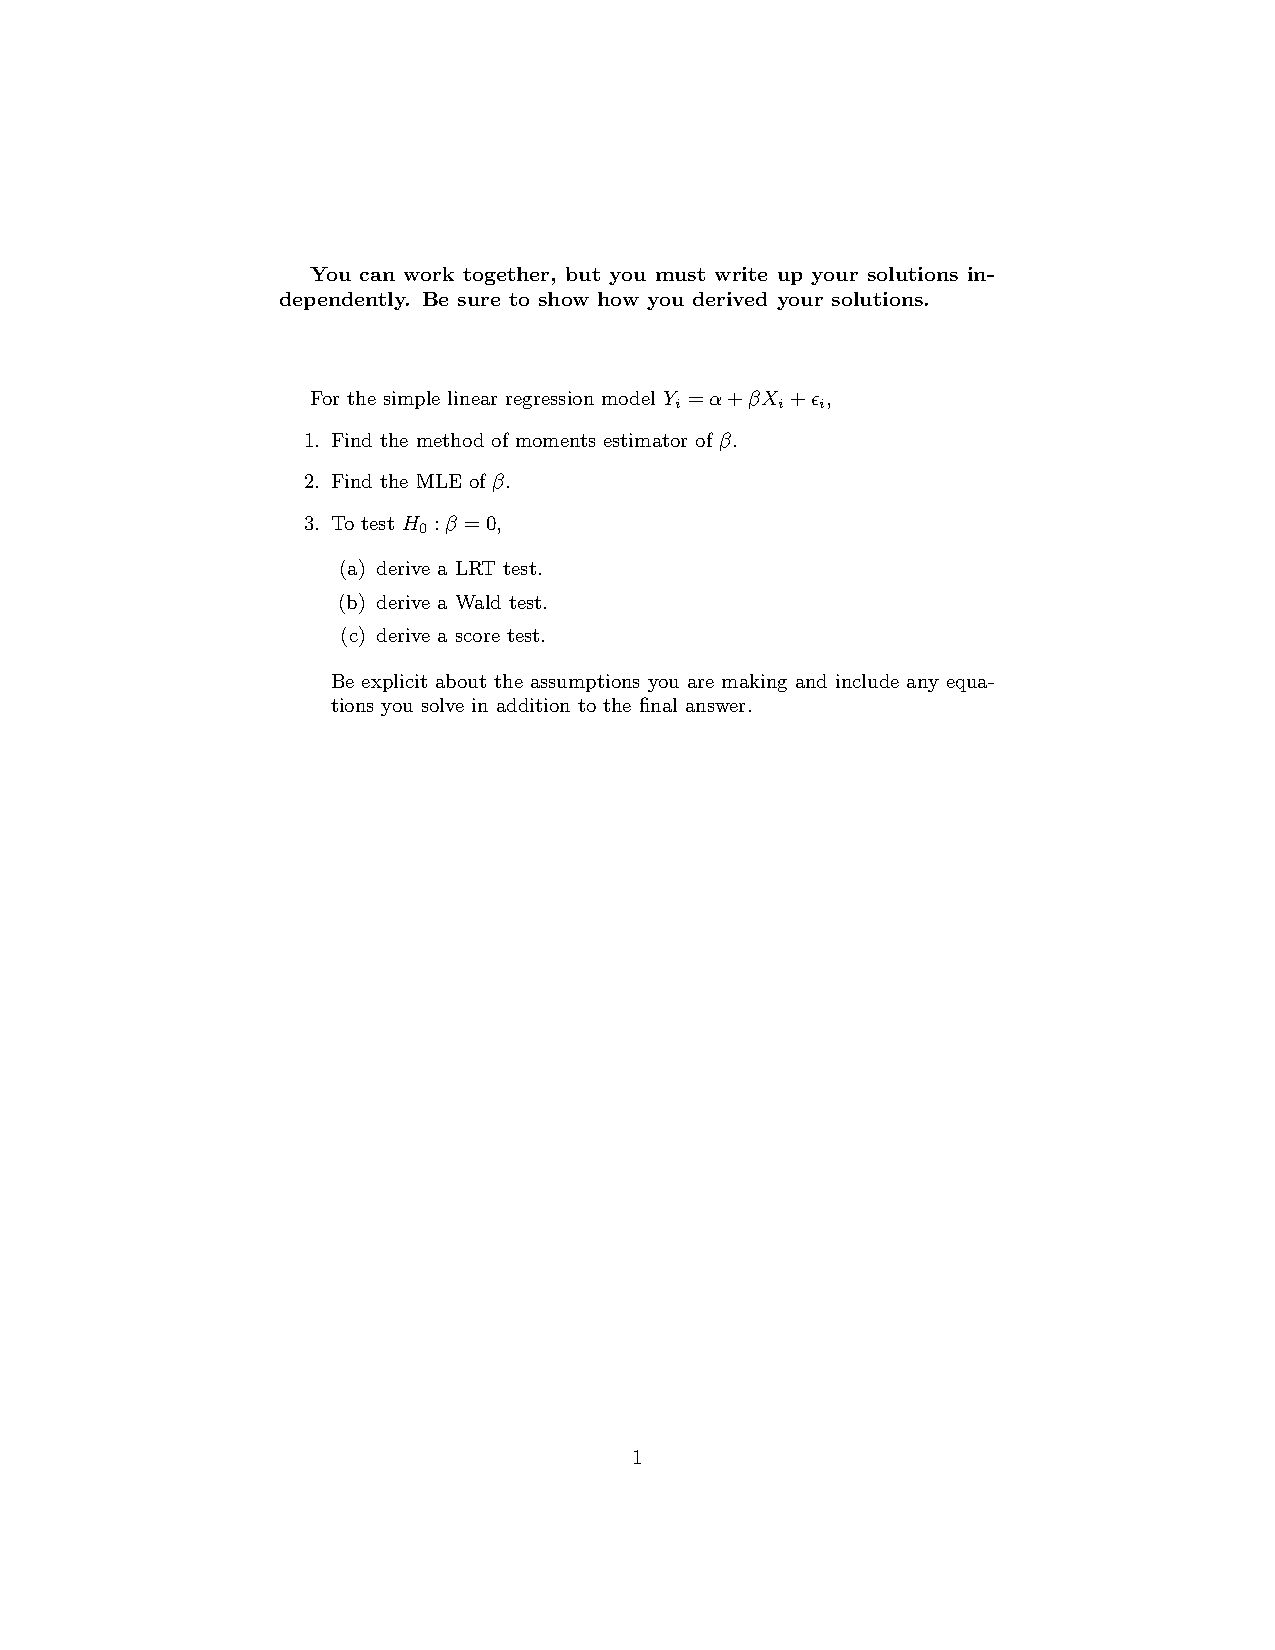
\includepdf[pages=-]{take_home_exam.pdf}
\maketitle

\begin{enumerate}
    \item
    Suppose $\alpha, \beta$ is parameters and $\epsilon_i, X_i$ are samples from two uncorrelated random variables, hence $Y_i$ are also samples from a random variables.
    Also we suppose $\epsilon_i$ have mean $0$ and $\frac{\sum{X^2_i}}{n} > (\frac{\sum{X_i}}{n})^2$.
    
    Then we have moments:
    \begin{eqnarray}
        \ep{Y} &=& \alpha + \beta \ep{X} + \ep{\epsilon} = \alpha + \beta \ep{X}\\
        \ep{X Y} &=& \alpha \ep{X} + \beta \ep{X^2} + \ep{\epsilon X} = \alpha \ep{X} + \beta \ep{X^2}
    \end{eqnarray} 
    Replace the expectation by the sample mean we have the MME of $\alpha, \beta$ are the solution of equation ($n$ is the sample size):
    \begin{eqnarray}
        \frac{\sum{Y_i}}{n} &=& \alpha + \beta \frac{\sum{X_i}}{n} \\
        \frac{\sum{X_i Y_i}}{n} &=& \alpha \frac{\sum{X_i}}{n} + \beta \frac{\sum{X_i^2}}{n} 
    \end{eqnarray}
    Then we solve that $\hat{\beta} = \frac{\overline{XY} - \overline{X} \cdot \overline{Y}}{\overline{X^2} - \overline{X}^2}$, where $\overline{X}, \overline{Y}, \overline{XY}, \overline{X^2}$ are the sample means of $X, Y, XY, X^2$.

    \item
    Suppose the sample size is $n$ and $(\epsilon_1, \epsilon_2, \cdots, \epsilon_n) \sim N(\bm{0}, \sigma^2 \textbf{I})$, where $\textbf{I}$ is the identity matrix of size $n \times n$. And $X_i$ are given numbers, $\sigma$ is known, $\alpha, \beta$ are parameters.
    Also suppose that $\frac{\sum{X^2_i}}{n} > (\frac{\sum{X_i}}{n})^2$.

    Then we have the likelihood of the sample is:
    $$L(\alpha, \beta) = \prod_1^n \frac{1}{\sqrt{2\pi}\sigma} \exp\{-\frac{(Y_i - \alpha - \beta X_i)^2}{2\sigma^2}\}$$
    Calculate the derivtives of $-\log{L(\alpha, \beta)}$, we get the regular equation for the MLE:
    \begin{eqnarray}
       \sum_1^n Y_i - \alpha - \beta X_i &=& 0 \\
       \sum_1^n X_i (Y_i - \alpha - \beta X_i) &=& 0
    \end{eqnarray}

    And the unique solution is indeed the minimal point of $-\log{L}$. Then we get that $\hat{\beta} = \frac{\overline{XY} - \overline{X} \cdot \overline{Y}}{\overline{X^2} - \overline{X}^2}$, where $\overline{X}, \overline{Y}, \overline{XY}, \overline{X^2}$ are the sample means of $X, Y, XY, X^2$.
    
    \item
    Here, we use the same assumption and notation as in question 2.
    \begin{enumerate}[(a)]
        \item 
        In this situation, the likelihood ratio is:
        $$\Lambda = \frac{\sup_{\alpha} L(\alpha, 0)}{\sup_{\alpha, \beta} L(\alpha, \beta)}$$

        The rejection field will be $\{\Lambda < C\}$, where $C$ is choosen by solve:
        $$ \{\sup_{\alpha} \prob{\Lambda < C | \alpha = \alpha, \beta = 0}\} = l_\alpha $$
        Where $l_\alpha$ is the level of the test you need.

        \item
        In this situation, the test statistics will be $T = \frac{(\hat{\beta} - 0)^2}{\var{\hat{\beta}}}$.
        And the rejection field will be $\{T > C\}$, where $C$ is choosen by solve:
        $$ \{\sup_{\alpha} \prob{T > C | \alpha = \alpha, \beta = 0}\} = l_\alpha $$
        Where $l_\alpha$ is the level of the test you need.

        \item
        In this situation, denote $\hat{\alpha}_0$ be the MLE of $\alpha$ when $\beta = 0$. And $U(\alpha, \beta)$ be the derivtive vector $\frac{\partial \log{L}(\alpha,\beta)}{\partial(\alpha, \beta)}$.
        And $I(\alpha, \beta)$ be the Fisher information matrix of this model.

        Then the test statistics is
        $$ S = U^T(\hat{\alpha}_0,0) I^{-1}(\hat{\alpha}_0,0) U(\hat{\alpha}_0,0) $$
        The rejection field is $\{S > C\}$, where $C$ is choosen by solve:
        $$ \{\sup_{\alpha} \prob{S > C | \alpha = \alpha, \beta = 0}\} = l_\alpha $$
        Where $l_\alpha$ is the level of the test you need.

    \end{enumerate} 

\end{enumerate}

\end{document}